{\bf BME154L - Spring 2012 - Exam \#2 Solutions}\hfill Name (Net ID):\underline{\hspace*{3.0in}}



\section{[70 points]}

Another approach to half-wave rectification is to utilize the ADC/DAC process instead of diodes.  We will work through this process in the following problem.  Consider a sinusoidal signal $f(t) = 5 \sin(2000 \pi t)$ V (Figure~\ref{fig:sig}(a)) and a desired output signal (a half-wave rectified input signal) (Figure~\ref{fig:sig}(b)):

\begin{figure}[htb!]
\begin{tabular}{cc}
\centering
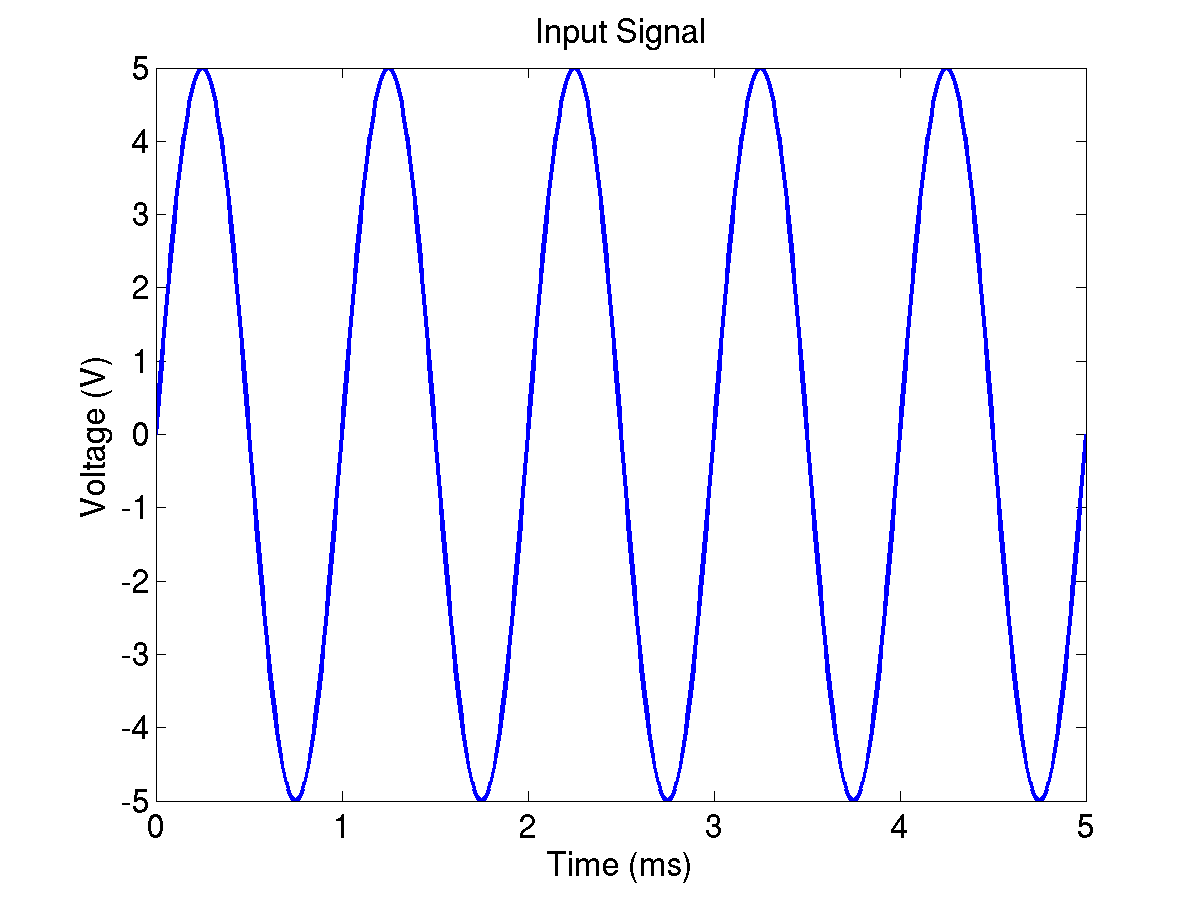
\includegraphics[width=0.5\linewidth]{in.png} &
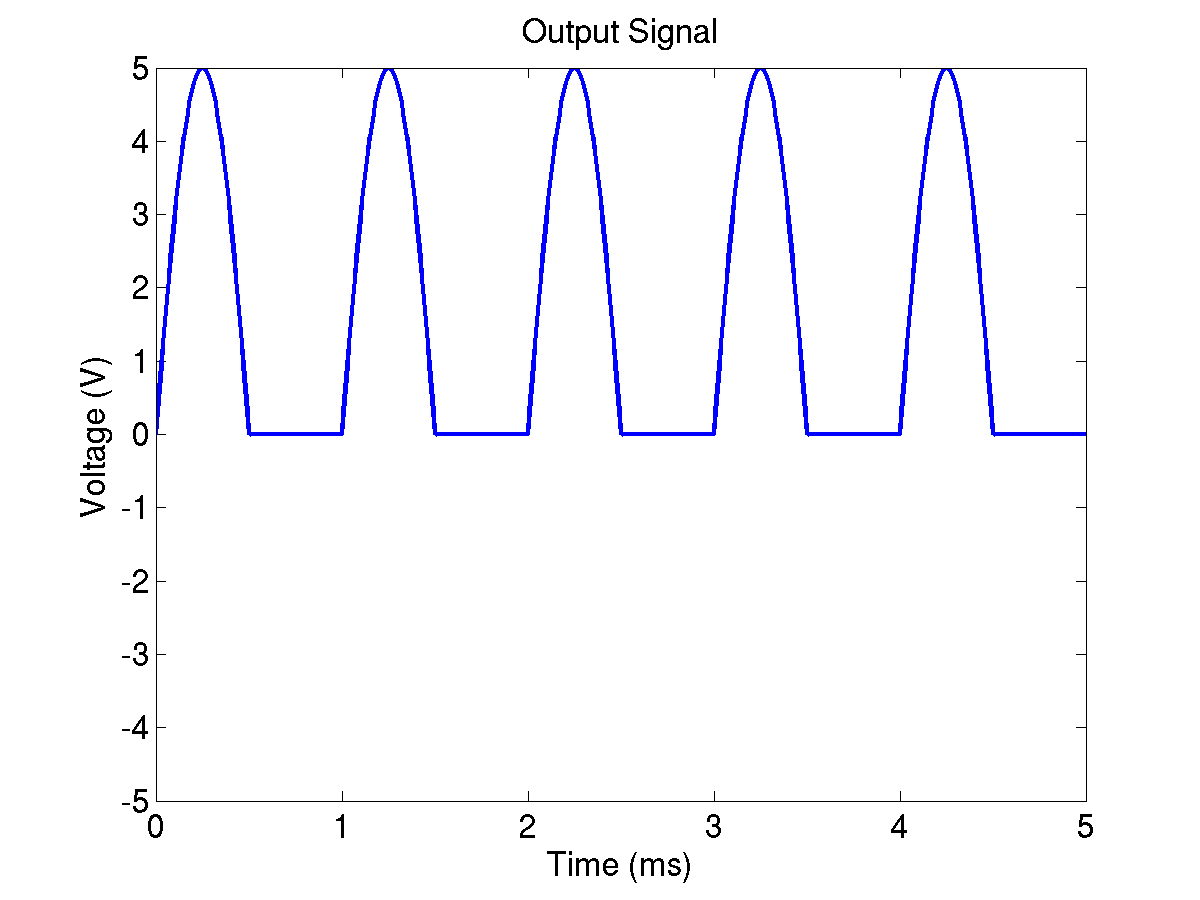
\includegraphics[width=0.5\linewidth]{out.png} \\
(a) Input Signal & (b) Output Signal \\
\end{tabular}
\caption{Input and Output Signals}
\label{fig:sig}
\end{figure}

\vspace*{0.5in}

We will use the following block diagram:

\vspace*{0.5in}

\begin{figure}[htb!]
\centering
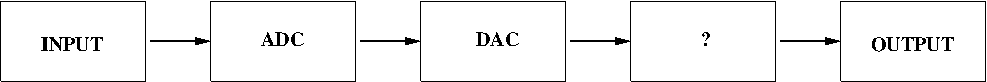
\includegraphics[width=0.75\linewidth]{block.png}
\caption{Block Diagram}
\label{fig:block}
\end{figure}

\clearpage

{\bf BME154L - Spring 2012 - Exam \#2 Solutions}\hfill Name (Net ID):\underline{\hspace*{3.0in}}



\begin{enumerate}

\item Sketch the power spectra of input (Figure~\ref{fig:sig}(a)) and output
(Figure~\ref{fig:sig}(b)) signals, labeling key features.\footnote{If you are having
trouble sketching these power spectra, then describe your thought process for
partial credit.} [10 points]

\item Some sampling frequency considerations:
\begin{itemize}
    \item What is the minimum sampling frequency of the ADC that you need to
faithfully reproduce the input signal to the DAC?  [5 points]
    \item What is the minimum DAC update frequency that you need to faithfully
reproduce the output signal?  Consider your answer to (a) and if there is any
benefit to updating your DAC output more frequently than the sampling frequency
of the ADC? [5 points]
\end{itemize}

\item Given an RMS white noise voltage of 0.5 V (not shown in
Figure~\ref{fig:sig}(a)), 
\begin{itemize}
    \item What is the SNR of the input signal? [5 points]
    \item What is the ideal number of bits that should be used
to sample the input signal to generate the desired output
signal?\footnote{``Ideal'' means the number of bits needed to fully represent
the signal without wasting bits sampling just noise.}\footnote{Hint: Saturation
of an ADC can be considered a design flaw in some circuits, but it can be taken
advantage of in this problem to remove parts of your input signal that you do
not want in your output signal.} [5 points]
\end{itemize}

\item Design the fastest ADC possible for this process.  Be sure to specify all
relevant component values. [10 points]

\item Successive Approximation ADC
\begin{itemize}
    \item If you were to use a successive approximation ADC for this problem, then
how many approximations would be needed for each binary number representation?  [5 points]
    \item Write a general expression that relates the minimum frequency of these
successive approximations to the sampling rate of the input signal such that there is no
loss of frequency content of the input signal. [5 points]
\end{itemize}

\item Design an R-2R DAC for your circuit. Be sure to specify all component values.  [10 points]

\item What error would be introduced into your DAC if the ``2R'' for your MSB
was 20\% greater than your ideal design?  (Provide a quantitative answer.) [5
points]

\item Design the ``?'' block in Figure~\ref{fig:block} to achieve the desired
output signal (Figure~\ref{fig:sig}(b)).  [5 points]

\end{enumerate}

\clearpage

{\bf BME154L - Spring 2012 - Exam \#2 Solutions}\hfill Name (Net ID):\underline{\hspace*{3.0in}}



\clearpage

{\bf BME154L - Spring 2012 - Exam \#2 Solutions}\hfill Name (Net ID):\underline{\hspace*{3.0in}}



\clearpage

{\bf BME154L - Spring 2012 - Exam \#2 Solutions}\hfill Name (Net ID):\underline{\hspace*{3.0in}}



\clearpage
